\documentclass[11pt,a4]{article}
\usepackage[slovene]{babel}
\usepackage{natbib}
\usepackage{url}
\usepackage[utf8x]{inputenc}
\usepackage{amsmath,amssymb,latexsym}
\usepackage{graphicx}
\usepackage{parskip}
\usepackage{fancyhdr}
\usepackage{vmargin}
\setmarginsrb{3 cm}{2.5 cm}{3 cm}{2.5 cm}{1 cm}{1.5 cm}{1 cm}{1.5 cm}

% Title
\title{Naslov naloge}
\date{\today}
\author{}

\makeatletter
\let\thetitle\@title
\let\theauthor\@author
\let\thedate\@date
\makeatother

\pagestyle{fancy}
\fancyhf{}
\rhead{\theauthor}
\lhead{\thetitle}
\cfoot{\thepage}

\begin{document}

%%%%%%%%%%%%%%%%%%%%%%%%%%%%%%%%%%%%%%%%%%%%%%%%%%%%%%%%%%%%%%%%%%%%%%%%%%%%%%%%%%%%%%%%%

\begin{titlepage}
	\centering
	\vspace*{-2cm}
    
\includegraphics[scale = 0.75]{logo_FPP.png}\\[1.0 cm]
    
	\rule{\linewidth}{1 mm} \\[0.4 cm]
	{ \huge \bfseries Ladijske elektronske naprave} \\[0.5 cm]
	{ \Large \bfseries Poročilo seminarske naloge}
	\rule{\linewidth}{1 mm} \\[1 cm]
	
	\rule{\linewidth}{0.5 mm} \\[0.4 cm]
	{ \large \bfseries \thetitle}\\[0.0 cm]
	\rule{\linewidth}{0.5 mm} \\[2 cm]
	
	\begin{minipage}{0.4\textwidth}
		\begin{flushleft} \large
			\emph{Avtorji naloge:}\\
			1. Študent Prvi\\
			2. Študent Drugi\\
			3. Študent Tretji
			\end{flushleft}
			\end{minipage}~
			\begin{minipage}{0.4\textwidth}
			\begin{flushright} \large
			\emph{Vpisna številka:} \\
			XXXXXX001\\
			XXXXXX002\\
			XXXXXX003									% Your Student Number
		\end{flushright}
	\end{minipage}\\[2 cm]
	
	\vfill
	
	{\large \thedate}\\[2 cm]
 
	
	
\end{titlepage}

%%%%%%%%%%%%%%%%%%%%%%%%%%%%%%%%%%%%%%%%%%%%%%%%%%%%%%%%%%%%%%%%%%%%%%%%%%%%%%%%%%%%%%%%%

\tableofcontents
\pagebreak

%%%%%%%%%%%%%%%%%%%%%%%%%%%%%%%%%%%%%%%%%%%%%%%%%%%%%%%%%%%%%%%%%%%%%%%%%%%%%%%%%%%%%%%%%

\section{Uvod}
To je splošna podlaga za poročilo seminarske nalog na \texttt{Fakulteti za pomorstvo in promet}. Ocena naloge se poda v \% (procentih).

Kazalo se v \LaTeX-u zgradi zmeraj samo. Imamo možnost različnih oblik fonta in izpisov znakov \textbf{je odebeljeno}. Literaturo enostavno citiramo z uporabo \texttt{\textbackslash cite\{\ldots\}} komande v našem  \texttt{yyyyyy.tex} dokumentu, torej citiram literaturo \cite{baker_1}. 

\subsection{Tabele in slike}
V \LaTeX vnašamo tudi tabele

\begin{table}[!htbp] 
	\caption{V tabeli so prikazani parametri mrež. Vse dolžinske mere so v milimetrih [mm]. (TET-tetraeder, HEX-heksaeder)}
	\vspace{2mm}
	\begin{center}
		{\small
			\begin{tabular}{c||l||c|c|c|c|c|c|c|c}\hline
				i & tip mreže & domain & fine box & vehicle & H$_1$  & $Y^+$ & Inflacijski model & layers & GR  \\ \hline \hline
				1 & TET + FLT & 20     & 4        & auto    & 0.01   & 1     & FLT               & 20     & 1.2 \\ \hline
				2 & TET + FLT & 20     & 4        & 0.6     & 0.01   & 1     & FLT               & 20     & 1.2 \\ \hline
				3 & TET       & 20     & 6        & 0.6     & -      & -     & brez              & -      & -   \\ \hline
				4 & TET       & 20     & 3        & auto    & -      & -     & brez              & -      & -   \\ \hline
				5 & TET + FAR & 15     & 5        & auto    & auto   & auto  & FAR               & 5      & 1.2 \\ \hline
				6 & HEX       & 15     & 7        & auto    & -      & -     & brez              & -      & -   \\ \hline
			\end{tabular}
		}
	\end{center}
	\label{tab:tabela_01}
\end{table}

in pa slike

\begin{figure}[!htbp]
	\centering 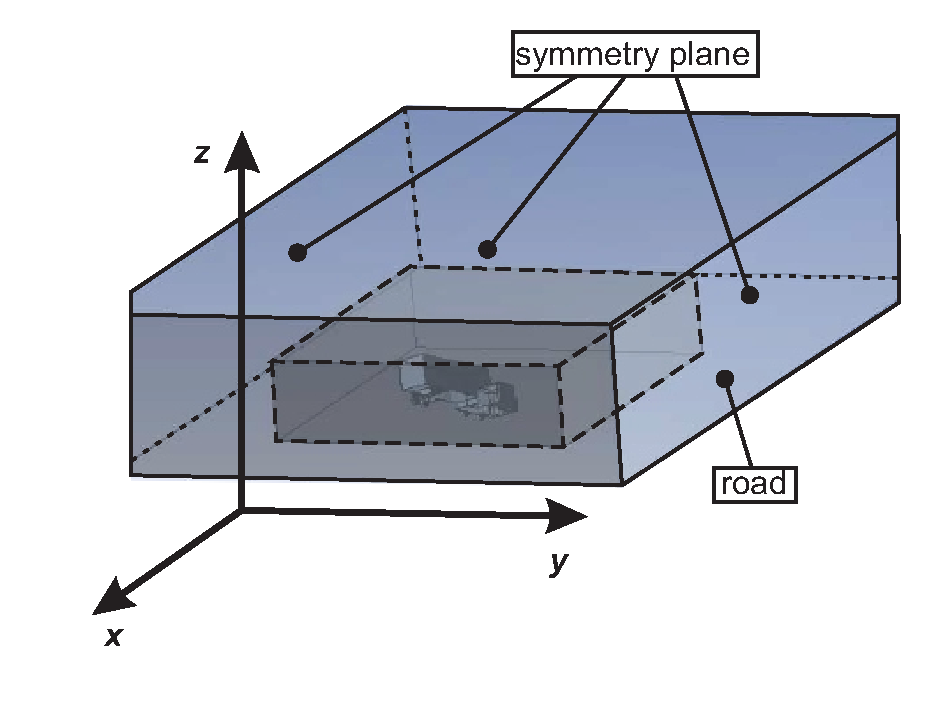
\includegraphics[width=6.5cm]{figs/geometry_3D.pdf}
	\caption{Prikaz postavitve računskega območja in označbe robnih pogojev. Lepo je vidna postavitev \emph{FineBox} subdomene, ki zaokoroža vozilo. Naš primer računa je za kot $\psi=0^\circ$.}
	\label{fig:slika_01}
\end{figure}

\newpage

in seveda slika 2

\begin{figure}[!htbp]
	\centering 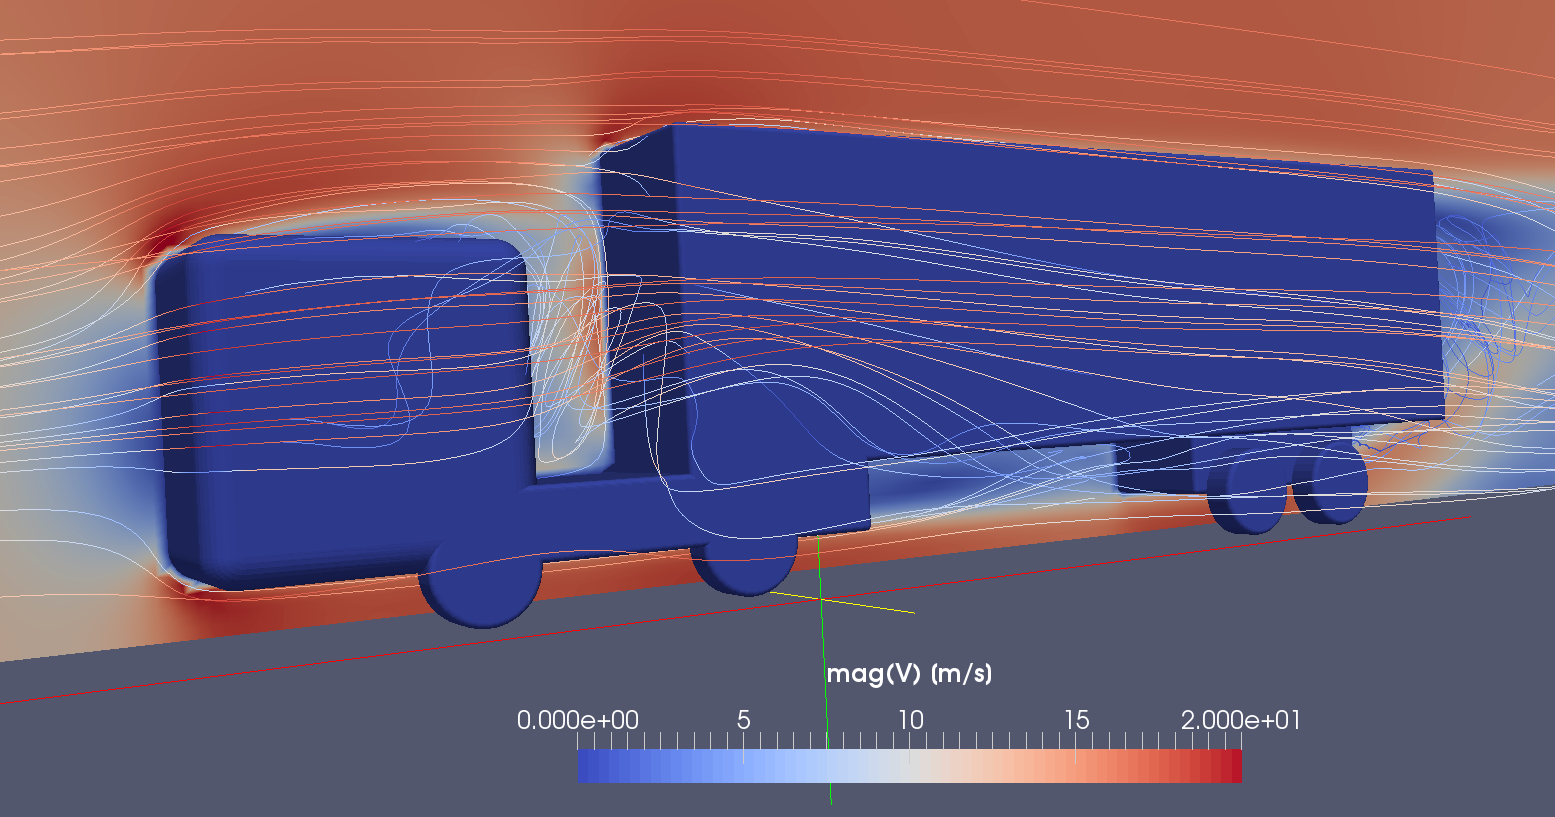
\includegraphics[width=6.5cm]{figs/res_L_01.png}
	\caption{Prikaz tokovnic in velikosti hitrosti ob vozilu.}
	\label{fig:slika_02}
\end{figure}

V tekstu se lahko enostavno sklicujemo na tabelo \ref{tab:tabela_01} in enako na sliko \ref{fig:slika_01} ali pa sliko \ref{fig:slika_02}.

\subsection{Enačbe}
Enako in zelo pomembno je pisanje enačb. Einstein je zapisal
\[
E = m \: c^2,
\]

bolj huda formula je pa
\[
I(x) = \int_0^x \frac{f(\zeta)}{g(\zeta)} d\zeta,
\]

in tako naprej.\\[1cm]

Veliko se o \LaTeX-u najde na:\\[0.2cm]
\url{https://www.latex-project.org/}\\
\url{https://en.wikibooks.org/wiki/LaTeX}\\[0.5cm]
Ostale stvari in nasvete glede \LaTeXe-a pa vse najdete na netu. 

\section{Citiranje literature}
Za vsako informacijo, sliko, podatek, ki je bil od nekod dobljen in ni vaše delo, je potrebno navesti vir. Kot smo že spoznali, vire navajamo s pomočjo komande \texttt{\textbackslash cite\{\ldots\}}. Vse vire shranimo in napišemo v datoteko \textit{literatura.bib} in potem vlečemo ven oz. navajamo vir s pomočjo ključa, recimo:\\
V teoriji mejne plasti \cite{boundary_layer_theory} je definirana konstanta Reynoldovega števila. Enako uporabljamo program za računanje tekočin \cite{openfoam} in navajamo internetni vir \cite{cfd_online_skin_friction}. Veliko informacij glede raziskav se nahajajo v člankih, ki jih citiramo \cite{bird_et_all}. Ja tako je s citiranjem.

\subsection{Instalacija \LaTeX okolja}
Celoten \LaTeX si v windows sistemu naložite z MikTex paketom, ki se nahaja na:\\[0.2cm]
\url{http://miktex.org/}\\[0.2cm]
Pazite, naložite si verzijo MikTex \texttt{verzija A.B.C.D} \textbf{NetInstaller} (32bit ali 64bit),\\[0.2cm]
kjer med inštalacijo izberete \textbf{Basic system}. V primeru, ko boste urejali besedilo (v TexStudiu) in bi potrebovali dodaten \LaTeX paket, vas bo MikTex sam opozoril in inštaliral paket direktno z neta.\\[0.5cm]

Za urejevalnik besedila priporočamo uporabo TexStudia:\\[0.2cm]
\url{https://en.wikibooks.org/wiki/LaTeX}


\newpage
\bibliographystyle{plain}
%\bibliographystyle{alpha}
\bibliography{literatura}

\end{document}